\input{../header.tex}

\subject{VERSUCH NUMMER 701}
\title{Reichweite von Alphastrahlung}
\date{
  Durchführung: 11.04.2023
  \hspace{3em}
  Abgabe: 18.04.2023
}

\begin{document}

\maketitle
\thispagestyle{empty}
\tableofcontents
\newpage
\setcounter{page}{1}
\section{Ziel}
\label{sec:Ziel}
\section{Theorie}
\label{sec:Theorie}


\section{Vorbereitungsaufgaben}
\label{sec:vorbereitung}

Ein Halbleiterzähler besteht aus je einem Halbleiter mit n-Leitung und p-Leitung. An der Kontaktstelle entsteht durch Diffusion eine Zone mit
beweglichen Ladungsträgern. Dies passiert solange bis das so aufgebaute elektrische Feld die weitere Diffusion verhindert. Der Übergang zwischen 
den Halbleitern ähnelt einer Diode. Wenn nun der n-Bereich mit einer Anode und der p-Bereich mit einer Kathode verbunden wird, vergrößert sich
der Bereich der freien Ladungsträger. Dieser Bereich wird auch Sperrzone genannt.

Wenn ein ionisierendes Teilchen durch diese Zone durchdringt, werden Elektronen und Löcher erzeugt. dadurch entsteht ein kurzzeitiger Stromfluss,
der messbar ist.
\section{Aufbau}
\label{sec:Aufbau}
Für die Messung der Reichweite von $\alpha$-Strahlen wird der in \autoref{fig:Aufbau} gezeigte Versuchsaufbau verwendet.
Die benötigten Bauteile sind eine Vakuumpummpe inklusive Druckmessgerät und Ventil, ein Vielkanalanalysator, einen luftdichten Glaszylinder mit Skala zur ABstandsmessung,
den Alphastrahler, einen in \autoref{sec:vorbereitung} beschriebenen Halbleiter-Detektor und einen Vorverstärker.
\begin{figure}
    \centering
    \includegraphics[height = 6cm]{Aufbau.pdf}
    \caption{Aufbau zur Messung der Reichweite von $\alpha$-Strahlen \cite{ap701}.}
    \label{fig:Aufbau}
\end{figure}
Die Bauteile werden ordnungsgemäß angeschlossen und die Messung kann Beginnen.

\section{Durchführung}
\label{sec:Durchführung}

Zunächst wird die Probe auf einen festen Abstand eingestellt und  die Kammer mithilfe der Vakuumpumpe evakuiert.
Wenn die Kammer einen Druck von $0\,\text{m}\unit{\bar}$ wird das Messprogramm auf dem Computer gestartet und die Messung beginnt. 
In den 2 Minuten die jede Messung durchgeführt wird, misst das Programm die Häufigkeit der Energien, die die Helium-Kerne besessen haben und hat als Ausgabe werden die Anzahl der 
detektierten $\alpha$-Teilchen, die häufigste Energie derer und die Häufigkeit dieser angezeigt.
Nach der Messung in der evakuierten Kammer wird der Druck in der Kammer auf $50\, \text{m}\unit{\bar}$ erhöht und ein erneuter Messdurchlauf gestartet.
Die Messung wird so lange fortgesetzt bis entweder ein Druck von $p= 1\, \unit{\bar}$ (welcher dem atmosphärischen Druck entspricht) erreicht ist oder keine Teilchen mehr nachgewiesen werden können.
Insgesamt werden so zwei Abstände ausgemessen.
Im Anschluss dazu wird die Statistik des radioaktiven Zerfalls untersucht.
Hierzu werden Druck, Temperatur und Abstand konstant gehalten und die Messung 100-mal wiederholt.
Gemessen wird 10 $\unit{\second}$ lang.
Es werden jeweils die Anzahl der detektierten Teilchen notiert, um später eine Aussage über die stochastische Verteilung der Häufigkeit von Zerfällen treffen zu können.

\section{Auswertung}
\label{sec:Auswertung}

\subsection{Fehlerrechnung}
\label{sec:Fehlerrechnung}
Für die Fehlerrechnung werden folgende Formeln aus der Vorlesung verwendet.
für den Mittelwert gilt
\begin{equation}
    \overline{x}=\frac{1}{N}\sum_{i=1}^N x_i ß\; \;\text{mit der Anzahl N und den Messwerten x} 
    \label{eqn:Mittelwert}
\end{equation}
Der Fehler für den Mittelwert lässt sich gemäß
\begin{equation}
    \increment \overline{x}=\frac{1}{\sqrt{N}}\sqrt{\frac{1}{N-1}\sum_{i=1}^N(x_i-\overline{x})^2}
    \label{eqn:FehlerMittelwert}
\end{equation}
berechnen.
Wenn im weiteren Verlauf der Berechnung mit der fehlerhaften Größe gerechnet wird, kann der Fehler der folgenden Größe
mittels Gaußscher Fehlerfortpflanzung berechnet werden. Die Formel hierfür ist
\begin{equation}
    \increment f= \sqrt{\sum_{i=1}^N\left(\frac{\partial f}{\partial x_i}\right)^2\cdot(\increment x_i)^2}.
    \label{eqn:GaussMittelwert}
\end{equation}

\subsection{Reichweite von Alphastrahlung}

Um die Reichweite von Alphastrahlung zu bestimmen muss der gemessene Channel des jeweiligen Drucks zuerst in MeV umgerechnet werden. Dabei entspricht der
Channel bei einem Druck $p = 0\,\symup{mbar}$ einer Energie $E = 4 \,\unit{\MeV}$. Diese fällt dann linear ab. Neben dem Druck, der Zählrate, dem 
Channel, der Energie und der Zählrate des jeweiligen Energiemaximums ist in \autoref{tab:3cm} auch noch die effektive Länge $x$ eingetragen. Diese
berechnet sich durch \autoref{eqn:effLaeng}. Die Messung wurde bei einem Abstand zwischen Detektor und Probe von $x_0 = 3\,\unit{\cm}$ durchgeführt.
\subsubsection{Erste Messreihe mit dem Abstand $x_0= 3\, \unit{\cm}$ vom Detektor}
\label{sec:Erste Messreihe}

\begin{table}
    \centering
    \caption{Druckabhängigkeit der Zählrate, der Energie und der effektiven Länge bei einem Abstand zwischen Probe und Detektor von $x_0 = 3\,\unit{\cm}$.}
\begin{tabular}{c c c c c c}
    \toprule
    $p \mathbin{/}\symup{mbar}$ &Zählrate& Channel & $E \mathbin{/}\symup{MeV}$ & Zählrate des Maximums & $x \mathbin{/}\unit{\m}$ \\
    \midrule
    0&55341&831&4.0000&190&0.0000 \\
    50&54428&816&3.9278&195&0.0015 \\
    100&53962&791&3.8075&201&0.0030\\
    150&53946&775&3.7304&213&0.0044\\
    200&52866&715&3.4416&234&0.0059\\
    250&52531&663&3.1913&234&0.0074\\
    300&51795&615&2.9603&242&0.0089\\
    350&51292&611&2.9410&263&0.0104\\
    400&50646&583&2.8063&252&0.0118\\
    450&49603&547&2.6330&256&0.0133\\
    500&48743&527&2.5367&276&0.0148\\
    550&47524&492&2.3682&261&0.0163\\
    600&45813&431&2.0746&268&0.0178\\
    650&42665&371&1.7858&278&0.0192\\
    700&36549&348&1.6751&283&0.0207\\
    750&24399&271&1.3045&288&0.0222\\
    800&15029&262&1.2611&256&0.0237\\
    850&3142&97&0.4669&262&0.0252\\
    900&92&6&0.0289&262&0.0267\\
    950&10&1&0.0048&274&0.0281\\
    1000&1&1&0.0048&259&0.0296\\
    \bottomrule
    \end{tabular}
    \label{tab:3cm}
\end{table}

Die letzten Messungen der Energie sind aufgrund der geringen Zählrate statistisch nicht mehr aussagekräftig.
\begin{figure}
  \centering
  \includegraphics[height= 8cm]{build/3cmeffLaeng.pdf}
  \caption{Graphische Auftragung der Zählrate gegen die effektive Länge bei dem Abstand 3 $\unit{\cm}$}
  \label{fig:3graph}
\end{figure}
\begin{figure}
  \centering
  \includegraphics[height= 8cm]{build/3cmenergie.pdf}
  \caption{Graphische Auftragung der Energie gegen die effektive Länge bei dem Abstand 3 $\unit{\cm}$}
  \label{fig:3energie}
\end{figure}
Zur Bestimmung des Energieverlust aus \autoref{eqn: energieverlust} wird eine Ausgleichskurve durch die Stelle des steilsten Abfalls gelegt werden (siehe \autoref{fig:3energie}).
Da diese Abnahme annähernd linear verläuft, wird eine Gerade der Form $f(x)=a\cdot x+b$ verwendet.
Die Parameter der Geraden konnten so als
\begin{align*}
  a&=-4.2054\,  \unit{\frac{\text{M}\electronvolt}{\meter}} \quad \text{und}\\
  b&= 127.0895\, \unit{\electronvolt}
\end{align*}
bestimmt werden.
Da $-\frac{\text{d}E}{\text{d}x}$, also die Änderung pro effektiver Länge gesucht ist, gilt
\begin{equation*}
  -\frac{\text{d}E}{\text{d}x}=-a=4.2054  \unit{\frac{\text{M}\electronvolt}{\meter}}
\end{equation*}


\subsubsection{Zweite Messreihe mit dem Abstand $x_0= 4.5\, \unit{\cm}$ vom Detektor}
Bei einer zweiten Messung wurde der Abstand zwischen Detektor und Probe auf $x_0 = 4.5 \,\unit{\cm}$ variiert. In \autoref{tab:4.5cm} sind erneut die 
Messdaten zu Zählrate, Channel, Energie, Zählrate des Energiemaximums sowie der effektiven Länge dargestellt.

\begin{table}
  \centering
  \caption{Druckabhängigkeit der Zählrate, der Energie und der effektiven Länge bei einem Abstand zwischen Probe und Detektor von $x_0 = 4.5\,\unit{\cm}$.}
\begin{tabular}{c c c c c c}
  \toprule
  $p \mathbin{/}\symup{mbar}$ &Zählrate& Channel & $E \mathbin{/}\symup{MeV}$ & Zählrate des Maximums & $x \mathbin{/}\unit{\m}$ \\
  \midrule
                    0&31206&830&4.0000&109&0.0000 \\
                    50&30522&768&3.7012&125&0.0022 \\
                   100&30102&745&3.5904&121&0.0044 \\
                   150&29734&675&3.2530&137&0.0067 \\
                   200&29168&668&3.2193&146&0.0089 \\
                   250&28700&631&3.0410&147&0.0111 \\
                   300&28323&559&2.6940&159&0.0133 \\
                   350&27222&536&2.5831&155&0.0155 \\
                   400&26401&463&2.2313&162&0.0178 \\
                   450&25624&412&1.9855&162&0.0200 \\
                   500&22454&367&1.7687&168&0.0222 \\
                   550&16202&295&1.4217&162&0.0244 \\
                     600&3458&271&1.3060&76&0.0267 \\
                       650&107&286&1.3783&6&0.0289 \\
                         700&7&462&2.2265&1&0.0311 \\
                         750&1&315&1.5181&1&0.0333 \\
                           800&0&0&0.0000&0&0.0355 \\
  \bottomrule
  \end{tabular}
  \label{tab:4.5cm}
\end{table}

\begin{figure}
  \centering
  \includegraphics[height= 8cm]{build/4.5cmeffLaeng.pdf}
  \caption{Graphische Auftragung der Zählrate gegen die effektive Länge bei dem Abstand 4.5 $\unit{\cm}$}
  \label{fig:4.5graph}
\end{figure}

\begin{figure}
  \centering
  \includegraphics[height= 8cm]{build/4.5cmenergie.pdf}
  \caption{Graphische Auftragung der Energie gegen die effektive Länge bei dem Abstand 4.5 $\unit{\cm}$}
  \label{fig:4.5energie}
\end{figure}

Die Berechnung des Energieverlust für den zweiten Abstand erfolgt ganz analog zu jener in \autoref{sec:Erste Messreihe}.
Die Parameter der Ausgleichsgeraden lassen sich zu
\begin{align*}
  a& = -3.4079\,  \unit{\frac{\text{M}\electronvolt}{\meter}}\quad \text{und}\\
  b&= 75.1149 \,  \unit{\electronvolt}
\end{align*}
berechnen. Die Gerade ist in \autoref{fig:4.5energie} dargestellt.
Für $-\frac{\text{d}E}{\text{d}x}$ folgt daraus
\begin{equation*}
  -\frac{\text{d}E}{\text{d}x}=-a = 3.4079\, \unit{\frac{\text{M}\electronvolt}{\meter}}\; .
\end{equation*}

\subsection{Vergleich beider Energieverluste}
Für $x_1= 3\,\unit{\cm} $ folgt $-\frac{\text{d}E}{\text{d}x}=4.2054 \, \unit{\frac{\text{M}\electronvolt}{\meter}}$ und für $x_2= 4.5\,\unit{\cm}$ folgt $-\frac{\text{d}E}{\text{d}x}=3.4079 \,\unit{\frac{\text{M}\electronvolt}{\meter}}$ .
Obwohl das Verhältnis von $x_1$ zu $x_2$ $\frac{2}{3}$ beträgt, stehen die Energieverluste im Verhältnis $\approx \frac{617}{500}=1.234$.
Es ist also zu erkennen, dass mit zunehmendem Abstand der Energieverlust geringer wird.

\subsection{Statistik des radioaktiven Zerfalls}
In \autoref{fig:histo} befindet sich das Histogramm zur gemessenen Statistik des radioaktiven Zerfalls.

\begin{figure}
  \centering
  \includegraphics[height = 6cm]{build/histo.pdf}
  \caption{Histogramm zur Statistik des radioaktiven Zerfalls.}
  \label{fig:histo}
\end{figure}

Der Mittelwert berechnet sich mittels \autoref{eqn:Mittelwert} zu $\overline{N} = 2443.23 \pm 9.49$. Die Varianz
der Messung liegt bei ${\Delta\overline{N}}^2 = 8913.197$.
In \autoref{fig:histo} sind neben der tatsächlichen Messwerte auch Normal- und Poissonverteilung eingezeichnet.
Zu sehen ist, dass die Normalverteilung viel näher an dem tatsächlichen Ausgang des Experiments liegt als die Poissonverteilung und somit 
anhand dieser bessere Vorhersagen über die Verteilung treffen kann.
\section{Diskussion}
\label{sec:Diskussion}


\newpage
\printbibliography
\nocite{ap308}
\nocite{matplotlib}
\nocite{numpy}
\nocite{scipy}
\nocite{uncertainties}
\nocite{reback2020pandas}

\newpage
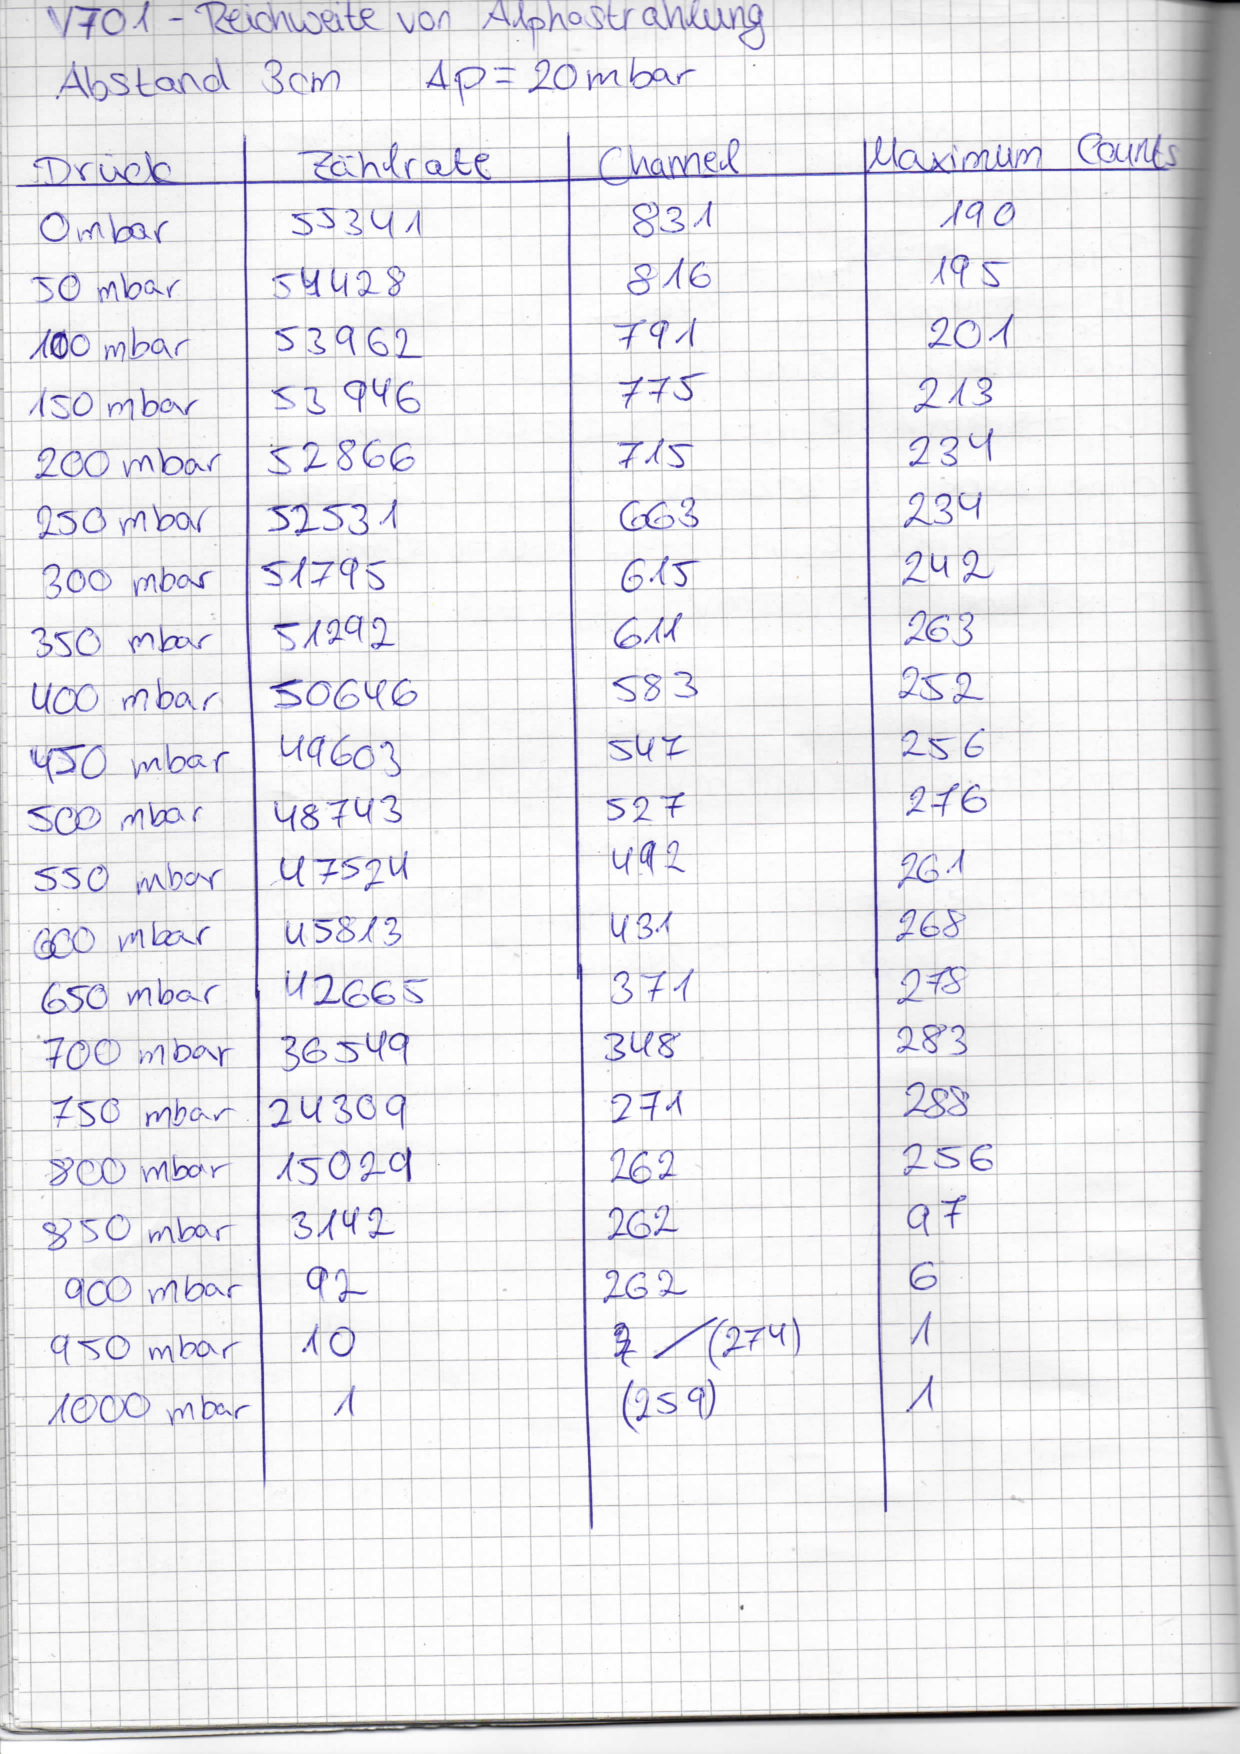
\includepdf[scale=0.7,pages=1,pagecommand=\section*{Anhang}\thispagestyle{empty}]{messdaten1.pdf}
\addcontentsline{toc}{section}{\protect\numberline{}Anhang}
\newpage
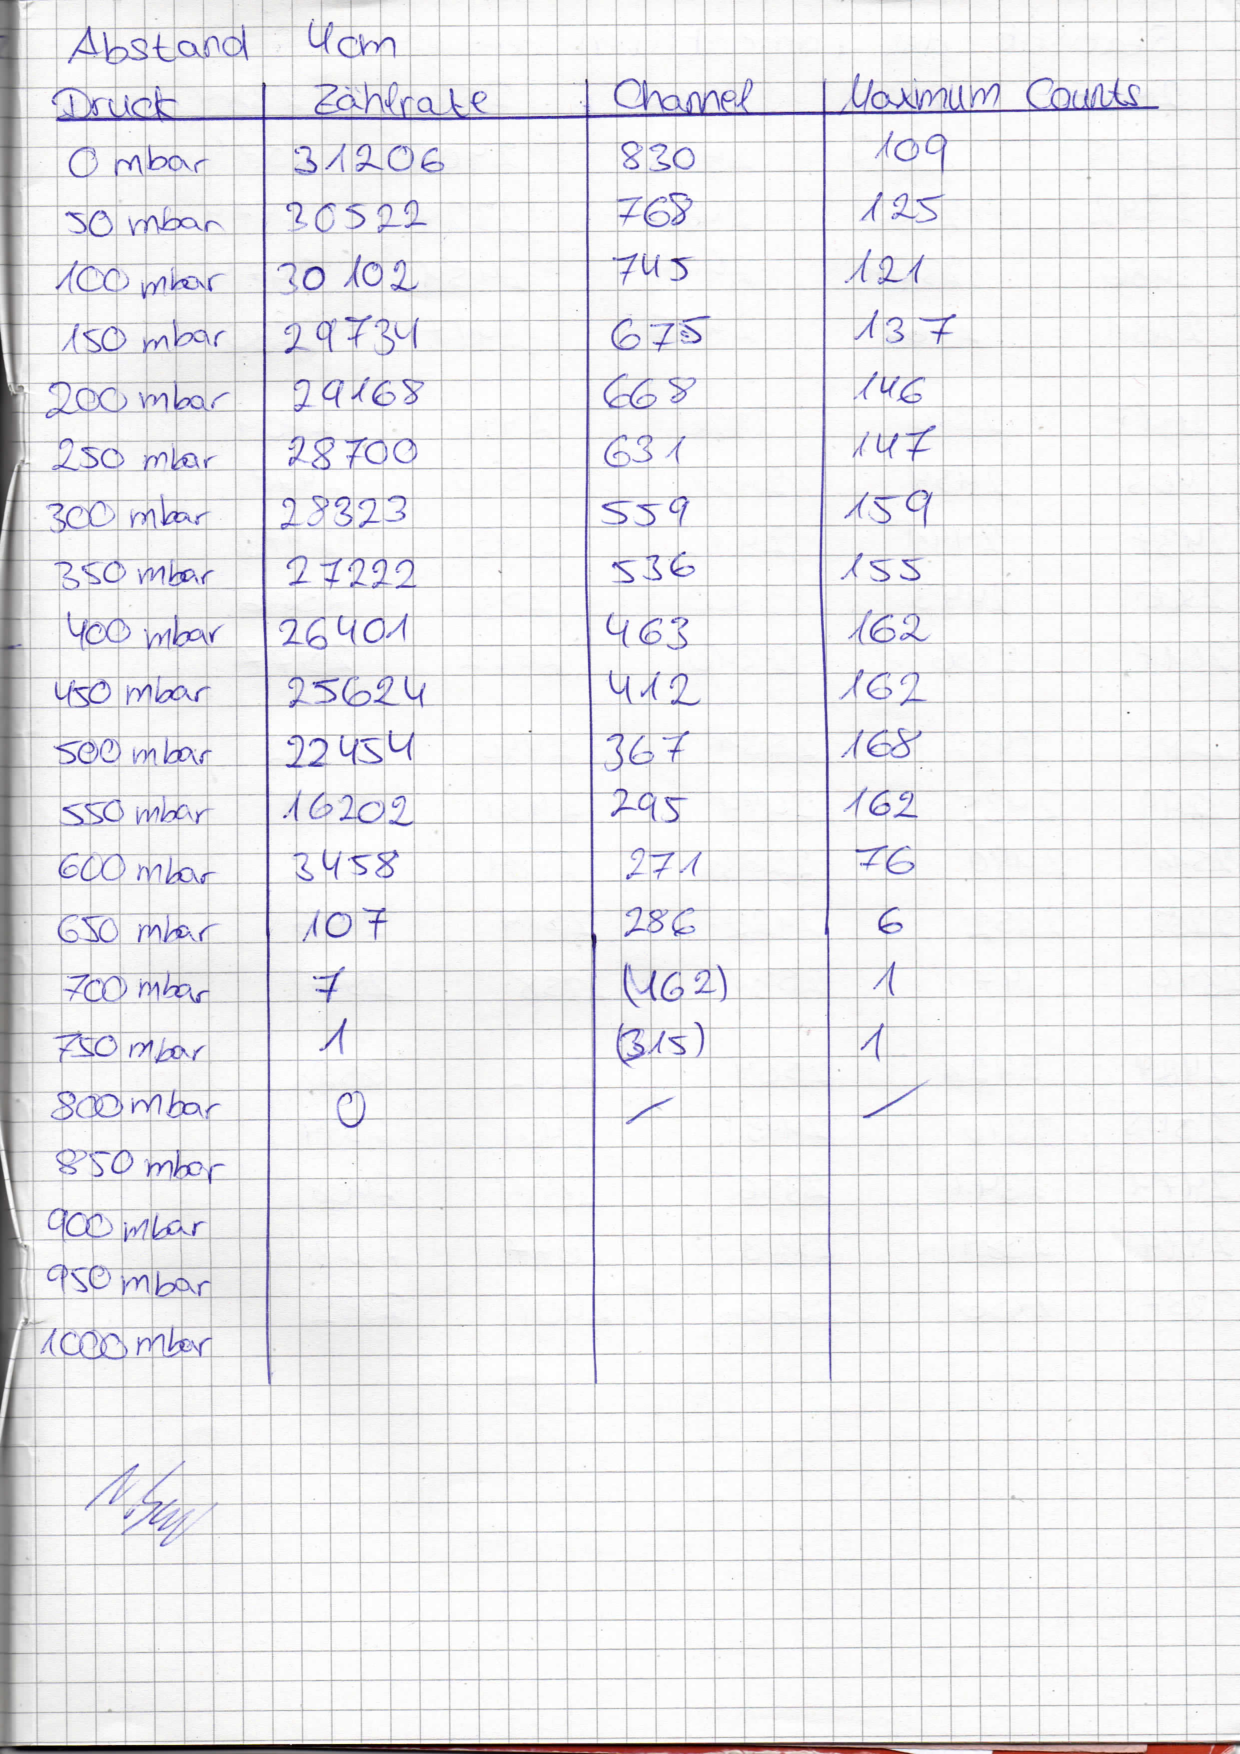
\includepdf[scale=0.7,pages=-]{messdaten2.pdf}

\end{document}
